\documentclass[conference]{IEEEtran}

\usepackage{cite}
\usepackage{amsmath,amssymb,amsfonts}
\usepackage{graphicx}
\usepackage{booktabs}
\usepackage{tabularx}
\usepackage{url}
\usepackage{xcolor}
\usepackage{tikz}
\usetikzlibrary{positioning, arrows.meta, fit, backgrounds}

\begin{document}

% Authors' note: Final paper title to be agreed upon by the team on Day 1.
\title{[TBD: Paper Title --- e.g., Score-Based Onboard Tile Prioritization for Emulated Satellite Imagery Pipelines]}

% Authors' note: Add institutional affiliation, department, city, country, and email addresses.
\author{
\IEEEauthorblockN{Vaibhav [TBD: Last Name], Ashutosh [TBD: Last Name], and Purnendu [TBD: Last Name]}
\IEEEauthorblockA{[TBD: Department, University, City, Country]\\
Email: \{[TBD: emails]\}}
}

\maketitle

% ============================================================================
% ABSTRACT (Owner: Vaibhav)
% ============================================================================
\begin{abstract}
% Authors' note: Replace [TBD] placeholders with measured results from E1--E5 and verify the exact framing once all experiments complete.
Earth-observation satellites generate high-resolution imagery faster than low-power onboard computers can process it or intermittent ground-station links can transmit it. Traditional bent-pipe pipelines transmit all captured data in acquisition order, preserving all information but delaying actionable results and consuming scarce downlink capacity on low-value regions such as clouds or open ocean. In this paper, we design and evaluate an emulated onboard satellite processing pipeline that streams multispectral Sentinel-2 imagery as fixed-size tiles, assigns each tile a low-cost priority score, and schedules processing and downlink under explicit onboard compute and bandwidth budgets. Our current implementation provides a parameterised simulation core, deterministic given fixed scorer costs, with byte-bounded input and priority queues, a pass-based downlink simulator, and two non-ML scorers (single-band variance and Sobel edge density) alongside random and FIFO baselines. We outline our planned integration with a windowed streaming tiler, a lightweight learned scorer, a containerized CPU/memory-capped execution environment, and a five-experiment evaluation against bent-pipe and oracle baselines. On [TBD: N] Sentinel-2 scenes, we will measure valuable-tile recall by deadline, time to deliver 90\% of valuable tiles, value density, onboard compute cost, and missed valuable tiles ([TBD: summary of headline E1--E5 results]). Because our setup emulates onboard hardware and replays processed Level-2A products, we report fidelity relative to an unconstrained heavy-model reference run rather than absolute ground truth, and leave sensor-level selective acquisition to future work.
\end{abstract}

\begin{IEEEkeywords}
orbital edge computing, satellite imagery, tile prioritization, priority scheduling, emulated onboard processing, Sentinel-2
\end{IEEEkeywords}

% ============================================================================
% I. INTRODUCTION (Owner: Vaibhav)
% ============================================================================
\section{Introduction}
% Owner: Vaibhav

% Authors' note: Verify the ESA PhiSat-1 sensor-vs-downlink growth rates and energy budget claim against full texts before submission.
Earth-observation satellites operate under two coupled resource bottlenecks: limited onboard compute and energy, and scarce satellite-to-ground downlink capacity. A pushbroom optical sensor sweeps the ground strip by strip as the satellite orbits, producing large multispectral scenes. As reported by the European Space Agency (ESA) PhiSat-1 team~\cite{phisat1} [VERIFY against full text], sensor data output grows roughly 100$\times$ per generation whereas downlink capability improves by only 3--5$\times$. At the same time, onboard processors are powered by solar panels and are substantially weaker than ground-based servers; as reported by Zhang et al.~\cite{targetfuse} [VERIFY against full text], an onboard computer cannot process every captured image within its harvested energy budget.

% Authors' note: Verify the bent-pipe prevalence, delay characterization, and PhiSat-1 cloud-filtering motivation against primary sources.
Most operational satellites follow a \emph{bent-pipe} architecture: they store raw imagery onboard, transmit it to ground stations during brief overhead contact windows, and defer all analysis to ground infrastructure [VERIFY against full text]. Bent-pipe transmission has an important property that any alternative must acknowledge: it never discards information. When downlink capacity is plentiful and latency is not critical, transmitting everything to the ground matches or outperforms onboard filtering. However, when contact windows are short, bandwidth is constrained, and users require timely information, bent-pipe delivery wastes scarce link capacity on uninformative data (such as cloud cover) and can delay useful results by hours or days. Conversely, running a heavy inference model on every captured tile onboard is infeasible when compute and energy budgets are tight.

% Authors' note: Confirm with the supervisor that onboard stream tiling after sensing (rather than sensor-level selective capture) matches project expectations.
A full satellite scene (such as a $60\times60$~km window or a $110\times110$~km Sentinel-2 granule at 10~m resolution [VERIFY against ESA documentation]) cannot be held entirely in memory on a small onboard computer. Instead, incoming imagery must be tiled as a stream and triaged incrementally. In this work, we investigate the following research question: \emph{Under fixed onboard compute and downlink budgets, does score-based tile prioritization deliver more valuable results, sooner, than processing tiles in capture order or downlinking all tiles sequentially?}

To study this question reproducibly without access to flight hardware, we are building an emulated onboard satellite pipeline that replays open Sentinel-2 Level-2A imagery as a tile stream, scores tiles using low-cost heuristics and a planned lightweight machine-learning (ML) model, and prioritizes tiles through byte-bounded queues and a simulated contact-window downlink. Because we cannot verify absolute ground truth across all scenes, we define the set of \emph{valuable} tiles $V$ via an explicit mission rule applied to an unconstrained heavy-model reference run; our evaluation therefore measures fidelity to full processing rather than ground-truth accuracy. Furthermore, we explicitly treat sensor-level selective acquisition---where the physical sensor skips regions prior to capture---as out of scope and future work.

Our contributions are as follows:
% Authors' note: Update the third contribution once Docker emulation, S3, and E1--E5 experiments are completed.
\begin{itemize}
    \item \textbf{Onboard Triage Simulator (Implemented):} We implement a seeded, parameterised pipeline core, deterministic given fixed scorer costs, comprising immutable multispectral tile records, a pluggable scorer registry with variance (S1), Sobel edge-density (S2), random, and FIFO baselines, a single-core compute-delay model with a byte-bounded FIFO input buffer, a byte-bounded evicting priority queue, and a non-overlapping contact-pass downlink simulator.
    \item \textbf{Streaming and Containerized Emulation (Planned):} We specify the integration of a windowed Sentinel-2 stream reader and SAHI-style tiler~\cite{sahi} inside a CPU- and memory-capped Docker container to emulate onboard resource limits without loading full scenes into memory.
    \item \textbf{Empirical Evaluation Framework (Planned):} We define five experiments (E1--E5) comparing cheap heuristics, a planned small ML scorer (S3), bent-pipe delivery, capture-order processing, and an oracle upper bound across [TBD: N] Sentinel-2 scenes, reporting both gains and missed valuable tiles [TBD: summary of findings].
\end{itemize}

% ============================================================================
% II. RELATED WORK (Owner: Vaibhav)
% ============================================================================
\section{Related Work}
% Owner: Vaibhav

% Authors' note: Verify OEC survey scope (2000--2023) and full citation details against arXiv:2306.00275.
Research on \emph{orbital edge computing} (OEC) moves part of the Earth-observation processing pipeline onto the satellite to reduce downlink waste and latency. A broad review of OEC research from 2000 to 2023 is provided by~\cite{oecsurvey} [VERIFY against full text]. In operational practice, ESA's PhiSat-1 mission demonstrated onboard AI-based cloud filtering to discard cloudy imagery before transmission, reportedly reducing download bandwidth demand by approximately 30\%~\cite{phisat1} [VERIFY against full text].

% Authors' note: Verify SAHI supported detectors and exact citation details against ICIP 2022 proceedings.
Processing high-resolution imagery on resource-constrained hardware requires dividing large scenes into manageable patches. Slicing Aided Hyper Inference (SAHI)~\cite{sahi} [VERIFY against full text] performs sliced inference by partitioning high-resolution images into smaller overlapping patches and supports standard object-detection frameworks. Rather than inventing a new slicing algorithm, our planned data ingestion layer adopts SAHI-style tiling with configurable patch size and overlap.

% Authors' note: Verify TargetFuse 3.4x error reduction and 9.6x bandwidth efficiency numbers against the IEEE INFOCOM 2024 full text.
Several recent systems combine onboard inference with prioritization under compute and downlink limits. TargetFuse~\cite{targetfuse} studies resource-efficient in-orbit object detection, arguing that an optimal tile size balances detection accuracy against computational overhead, and uses clustering-based deduplication alongside model confidence scores to prioritize downlink transmission. Under a bandwidth budget, TargetFuse reports 3.4$\times$ lower detection error than onboard computing alone and 9.6$\times$ better bandwidth efficiency than a vanilla baseline~\cite{targetfuse} [VERIFY against full text].

% Authors' note: Verify Kodan full author list, exact mechanism, and data value density definition against ASPLOS 2023 full text.
Kodan~\cite{kodan} addresses the computational bottleneck in space by filtering low-value imagery and prioritizing high-value data, reporting gains in data value density [VERIFY against full text]. EarthSight~\cite{earthsight} predicts priorities and allocates compute budgets to incoming satellite imagery, rejecting low-value images early to achieve low-latency intelligence [VERIFY against full text]. An alternative approach to the downlink bottleneck is neural feature compression, as explored by FOOL~\cite{fool} [VERIFY against full text], which compresses intermediate representations rather than filtering or reordering tiles.

% Authors' note: Verify this gap statement against the full texts of TargetFuse, Kodan, and EarthSight before final submission.
\textbf{Research Gap.} Existing OEC systems such as TargetFuse~\cite{targetfuse}, Kodan~\cite{kodan}, and EarthSight~\cite{earthsight} demonstrate onboard filtering, priority prediction, and compute-budget allocation within their respective system designs. However, [VERIFY against full texts] there remains a need for an open, reproducible emulated pipeline that systematically compares ultra-cheap non-ML heuristics against a lightweight learned scorer and priority scheduling policies under identical, explicit compute and downlink budgets, while accounting for scorer overhead (dropped unscored tiles) and reporting missed valuable tiles alongside latency and bandwidth gains.

% ============================================================================
% III. DATA AND TILING (Owner: Vaibhav)
% ============================================================================
\section{Data and Tiling}
% Owner: Vaibhav

% Authors' note: Verify Sentinel-2 technical specifications (altitude, swath, band count, granule size, and L2A reflectance scaling offset) against official ESA documentation.
\subsection{Sentinel-2 Imagery (Planned)}
Our planned dataset consists of [TBD: 20--50] open Sentinel-2 Level-2A scenes from ESA's Earth-observation mission. Sentinel-2 carries a pushbroom multispectral instrument at 786~km altitude with a 290~km swath and 13 spectral bands, four of which have 10~m spatial resolution: B02 (blue), B03 (green), B04 (red), and B08 (near-infrared) [VERIFY against ESA documentation]. Standard Sentinel-2 Level-2A products are $110\times110$~km ortho-images ($10{,}980\times10{,}980$ pixels at 10~m resolution), referred to by ESA as \emph{granules} [VERIFY against ESA documentation]. Throughout this paper, we use \emph{granule} for the ESA product unit and \emph{tile} for our smaller square crops.

% Authors' note: Fill in exact scene list, geographic distribution, cloud-cover breakdown, and train/val/test split counts once scenes are downloaded.
We plan to select scenes covering a diverse mix of land-cover types---including urban/industrial areas, farmland, desert, ocean, and varying cloud cover---so that tile value varies substantially within and across scenes ([TBD: scene count, geographic regions, and date range]). Scenes will be partitioned strictly \emph{by scene} (e.g., [TBD: 60\% train, 20\% validation, 20\% test, with at least 4 held-out test scenes]) rather than by tile, preventing spatial data leakage between adjacent tiles. Because Level-2A products are already radiometrically and atmospherically corrected on the ground, replaying them as a live onboard stream is an explicit simplification; we will also verify and apply the product's reflectance scaling and any processing-baseline offset consistently ([TBD: exact ESA baseline and offset handling]; note that an additive offset does not affect S1 variance or S2 Sobel gradients, only the scale divisor and S3's NDVI/NDWI).

\subsection{Windowed Streaming and Tiling (Planned)}
% Authors' note: Replace placeholders with implemented rasterio windowed-read parameters, tile size, overlap, padding, and nodata handling once Role C completes the tiler.
To respect onboard memory limits without holding a full granule in RAM, our planned ingestion module will read horizontal strips of rows from disk using windowed reads (e.g., via \texttt{rasterio}) and slice each strip into square tiles following SAHI-style slicing~\cite{sahi}. Planned configuration parameters include tile size ([TBD: e.g., $256\times256$ pixels, covering $2.56\times2.56$~km at 10~m resolution, or matched to the heavy model's input size]), overlap ([TBD: overlap fraction/pixels]), border padding, and nodata filtering ([TBD: exact nodata rule]).

In the current codebase, the ingestion boundary is defined by an implemented \texttt{TileSource} abstraction that yields immutable \texttt{Tile} records in capture order. Each \texttt{Tile} contains a $(H, W, C)$ \texttt{uint16} pixel array, ordered band names \texttt{(B02, B03, B04, B08)}, a simulated capture timestamp, and its size in bytes. Once completed, the windowed streaming tiler will plug directly into \texttt{TileSource} without modifying downstream pipeline components.

% ============================================================================
% IV. SCORING METHODS AND REFERENCE DEFINITION (Owner: Ashutosh)
% ============================================================================
\section{Scoring Methods and Reference Definition}
% Owner: Ashutosh

\subsection{Scorer Interface (Implemented)}
Every tile arriving at the onboard triage layer is evaluated by a scorer implementing a uniform interface:
\begin{equation}
    \text{score}(\text{tile}) \rightarrow s \in \mathbb{R},
\end{equation}
where higher values of $s$ indicate a higher predicted priority for processing and downlink. Scores are comparable only within a single scorer; only the relative ranking among tiles affects queue eviction and transmission order. The pipeline measures the wall-clock execution time of each \texttt{score} call per tile, and a pluggable scorer registry allows new scorers (including external ML models) to be registered without modifying the pipeline core.

\subsection{Implemented Heuristic Scorers and Baselines}
Four scoring mechanisms are currently implemented and verified in the codebase:
\begin{itemize}
    \item \textbf{S1 (Single-Band Variance):} Computes the pixel variance of a single band (defaulting to near-infrared \texttt{B08}) in \texttt{float64} precision. The intuition is that homogeneous regions such as open water or uniform cloud decks exhibit low pixel variance, whereas structured terrain or built-up areas exhibit higher variance.
% Authors' note: Calibrate the S2 Sobel gradient magnitude threshold (currently placeholder 0.02) on real Sentinel-2 tiles and report the final value.
    \item \textbf{S2 (Sobel Edge Density):} Scales the selected band by dividing raw \texttt{uint16} values by $10{,}000$, computes the Sobel gradient magnitude per pixel, and returns the fraction of pixels whose gradient magnitude exceeds a threshold $\tau$. The current default $\tau = 0.02$ is a [TBD: placeholder threshold to be calibrated on real Sentinel-2 tiles]. A mean-gradient-magnitude variant of S2 is also implemented for ablation studies.
    \item \textbf{Random Baseline:} Assigns a pseudo-random score derived from the run seed and the tile identifier, establishing a lower-bound ordering baseline.
    \item \textbf{FIFO Baseline:} Assigns priority strictly by capture order (earlier capture timestamp first), modeling order-preserving sequential handling without content-based prioritization.
\end{itemize}

\subsection{Planned Small ML Scorer (S3)}
% Authors' note: Complete S3 feature list, model family, GroupKFold tuning details, and training set size once Ashutosh completes Steps 5--7.
To evaluate whether a lightweight learned predictor outperforms hand-crafted heuristics, we plan to implement a small ML scorer (S3) registered via the existing scorer registry. S3 will extract low-cost per-tile features---including per-band means and standard deviations (\texttt{B02}, \texttt{B03}, \texttt{B04}, \texttt{B08}), overall brightness, pixel variance, Sobel edge density, vegetation and water indices ($\text{NDVI} = (\text{B08}-\text{B04})/(\text{B08}+\text{B04})$ and $\text{NDWI} = (\text{B03}-\text{B08})/(\text{B03}+\text{B08})$), and bright-pixel fraction as a cloud proxy---and train a compact classifier (starting with class-balanced logistic regression and evaluating tree-based ensembles such as \texttt{HistGradientBoostingClassifier}) using \texttt{GroupKFold} grouped by \texttt{scene\_id} ([TBD: final S3 model choice, hyperparameters, and per-tile inference cost]).

\subsection{Mission Rule and Reference Definition (Planned)}
% Authors' note: Insert the frozen MISSION.md rule, heavy model checkpoint, license, input size, and prevalence of V once finalized on Day 1.
To evaluate prioritization objectively, we will first freeze a mission rule in \texttt{MISSION.md} defining which land-cover classes constitute valuable imagery (e.g., urban and infrastructure classes such as Residential, Industrial, and Highway with combined confidence above a fixed threshold [TBD: exact mission rule and threshold]). We will then run an unconstrained reference pass using a pretrained land-cover classification model ([TBD: heavy model name, checkpoint, input size, and bands]) over every tile of every scene. The set of tiles flagged by this reference run defines the valuable set $V$.

We emphasize that $V$ represents \emph{fidelity to unconstrained heavy-model processing}, not absolute physical ground truth. The mission rule will be frozen prior to inspecting any scorer results on validation or test scenes, and the scene mix will be checked to ensure $V$ represents a meaningful minority of tiles ([TBD: target prevalence, e.g., 10--40\%]).

% ============================================================================
% V. SYSTEM DESIGN (Owner: Purnendu)
% ============================================================================
\section{System Design}
% Owner: Purnendu

\begin{figure*}[t]
\centering
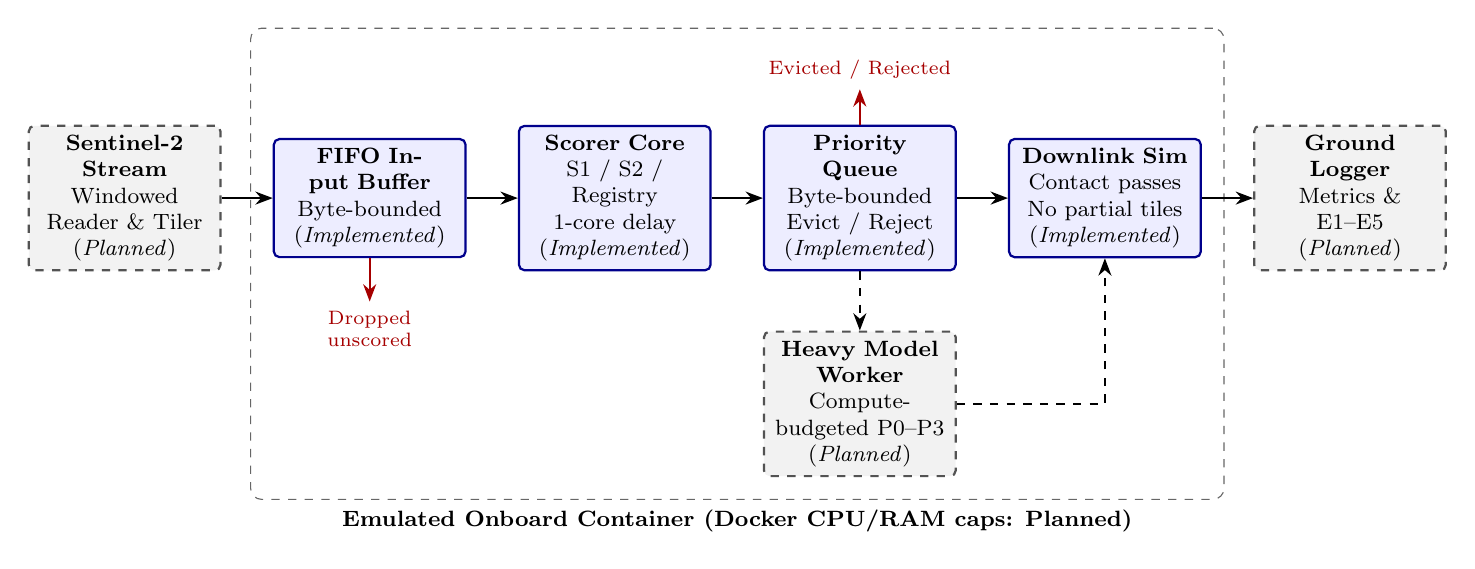
\begin{tikzpicture}[
    node distance=0.55cm and 0.65cm,
    box/.style={draw, rectangle, rounded corners=2pt, minimum height=1.15cm, text width=2.2cm, align=center, font=\footnotesize},
    impl/.style={box, fill=blue!7, draw=blue!55!black, thick},
    plan/.style={box, fill=gray!10, draw=gray!65!black, dashed, thick},
    arr/.style={-{Stealth[length=2.2mm]}, thick}
]
    % Nodes
    \node[plan] (source) {\textbf{Sentinel-2 Stream}\\Windowed Reader \& Tiler\\(\textit{Planned})};
    \node[impl, right=of source] (inbuf) {\textbf{FIFO Input Buffer}\\Byte-bounded\\(\textit{Implemented})};
    \node[impl, right=of inbuf] (scorer) {\textbf{Scorer Core}\\S1 / S2 / Registry\\1-core delay\\(\textit{Implemented})};
    \node[impl, right=of scorer] (pq) {\textbf{Priority Queue}\\Byte-bounded\\Evict / Reject\\(\textit{Implemented})};
    \node[impl, right=of pq] (dl) {\textbf{Downlink Sim}\\Contact passes\\No partial tiles\\(\textit{Implemented})};
    \node[plan, right=of dl] (ground) {\textbf{Ground Logger}\\Metrics \& E1--E5\\(\textit{Planned})};

    % Planned heavy model branch
    \node[plan, below=0.75cm of pq] (heavy) {\textbf{Heavy Model Worker}\\Compute-budgeted P0--P3\\(\textit{Planned})};

    % Drop / Evict annotations
    \node[below=0.55cm of inbuf, font=\scriptsize, align=center, text=red!65!black] (drop) {Dropped\\unscored};
    \node[above=0.45cm of pq, font=\scriptsize, align=center, text=red!65!black] (evict) {Evicted / Rejected};

    % Arrows
    \draw[arr] (source) -- (inbuf);
    \draw[arr] (inbuf) -- (scorer);
    \draw[arr] (scorer) -- (pq);
    \draw[arr] (pq) -- (dl);
    \draw[arr] (dl) -- (ground);
    \draw[arr, dashed] (pq) -- (heavy);
    \draw[arr, dashed] (heavy) -| (dl);
    \draw[arr, red!65!black] (inbuf) -- (drop);
    \draw[arr, red!65!black] (pq) -- (evict);

    % Container boundary
    \begin{scope}[on background layer]
        \node[draw=black!60, dashed, rounded corners=4pt, inner sep=8pt,
              fit=(inbuf) (scorer) (pq) (dl) (heavy) (drop) (evict),
              label={[font=\footnotesize\bfseries]below:Emulated Onboard Container (Docker CPU/RAM caps: Planned)}] {};
    \end{scope}
\end{tikzpicture}
\caption{Architecture of the emulated onboard tile prioritization pipeline. Solid blue blocks indicate implemented components; dashed gray blocks indicate planned components (windowed streaming tiler, heavy-model worker, containerized resource caps, and ground-side metric aggregation).}
\label{fig:arch}
\end{figure*}

Figure~\ref{fig:arch} shows the end-to-end architecture of our emulated onboard pipeline, clearly distinguishing implemented simulation components from planned integration modules. All runs are deterministic given fixed scorer costs, seeded, and parameterised. Experiments use a calibrated cost table (median per-scorer time from the timing harness, times the speed factor) supplied as a fixed cost, because raw wall-clock timings vary between runs; measured timings are reported separately.

\subsection{Implemented Pipeline Core}
The implemented simulator models the arrival, scoring, buffering, and downlink transmission of tiles using discrete event times:

\paragraph{Input Buffer and Single-Core Compute Model}
Tiles arrive from a \texttt{TileSource} in capture order. Incoming tiles first enter a byte-bounded FIFO input buffer. If the buffer lacks sufficient free capacity in bytes for an arriving tile, that tile is immediately marked \emph{dropped unscored}. A single simulated compute core dequeues tiles from the input buffer and executes the configured scorer. Scoring a tile advances the core's simulated clock by
\begin{equation}
    t_{\text{score}} = c_{\text{measured}} \times \alpha,
\end{equation}
where $c_{\text{measured}}$ is the measured wall-clock scoring time and $\alpha$ is a configurable speed factor representing slower onboard hardware. Once scoring finishes, the tile is submitted to the priority queue. This model captures a key systems trade-off: an expensive scorer occupies the core longer, causing the input buffer to fill and incoming tiles to be dropped unscored.

\paragraph{Byte-Bounded Priority Queue}
Scored tiles enter a priority queue whose capacity is bounded in \emph{bytes} rather than tile count. Ordering is determined lexicographically by: (1) higher priority score, (2) earlier capture timestamp, and (3) smaller tile identifier. When a newly scored tile arrives and the queue lacks sufficient free bytes, the queue checks whether enough lower-priority bytes can be freed to admit the new tile. Tiles are evicted (and recorded as \emph{evicted}) only if enough lower-priority bytes can be freed to admit the new tile; otherwise, nothing is evicted and the new tile is rejected (recorded as \emph{rejected}).

\paragraph{Contact-Pass Downlink Simulator}
Downlink transmission is modeled as a sorted list of non-overlapping contact passes, each specified by a start time, duration, and bandwidth (bytes per second). During an active pass, the simulator pops the highest-ranked tile from the priority queue and transmits it if and only if the tile fits \emph{entirely} within the remaining pass capacity (no partial-tile transmission). If the top-ranked tile does not fit in the remaining capacity of the current pass, the pass terminates immediately (head-of-line blocking). For each delivered tile, delivery time accounts for cumulative transmission time within the pass ($\text{cumulative bytes} / \text{bandwidth}$).

\paragraph{Complete Tile Accounting and Timing Harness}
At the end of a simulation run, every tile emitted by the \texttt{TileSource} is accounted for in exactly one of five mutually exclusive outcome categories: \emph{delivered} (with recorded end-to-end delay), \emph{evicted}, \emph{rejected}, \emph{still-in-queue}, or \emph{dropped-unscored}. To benchmark scorer latency and memory cleanly, we also implement a dedicated timing harness that performs warm-up iterations followed by repeated timed runs, reporting median and p95 latency, while measuring memory usage in a separate pass to avoid profiler distortion of latency measurements.

\subsection{Planned Components}
% Authors' note: Update this subsection to past tense once Docker caps, heavy-model worker, and P0--P3 policies are implemented.
Four system components are planned for integration prior to running full experiments:
\begin{enumerate}
    \item \textbf{Containerized Resource Emulation:} Wrapping the pipeline inside a Docker container with explicit CPU and memory caps (planned baseline profile: [TBD: e.g., 2 vCPU and 2~GB RAM]) to emulate a constrained onboard computer.
    \item \textbf{Heavy-Model Worker and Policies P0--P3:} Extending the current runner (which supports scorer-driven ordering alongside random and FIFO baselines) to execute the four comparison policies defined in our project plan: \textbf{P0 (Bent Pipe)}, transmitting raw tiles in capture order with no onboard inference; \textbf{P1 (Process-Everything Onboard)}, running the heavy model in capture order until the compute budget is exhausted; \textbf{P2 (Score-and-Skip)}, skipping tiles below a validation-chosen score threshold; and \textbf{P3 (Priority Processing and Downlink)}, allocating both heavy-model compute and downlink capacity in priority order. An \textbf{Oracle} upper bound that transmits exactly the tiles in $V$ will also be implemented.
    \item \textbf{Ground-Side Metrics and Experiment Runner:} Automated batch execution over all scenes and budget sweeps using YAML run configurations, computing recall, latency, value density, and miss metrics, and generating plots.
    \item \textbf{Real-Scene Integration:} Connecting the windowed Sentinel-2 tiler to \texttt{TileSource} and registering the trained S3 scorer.
\end{enumerate}

% ============================================================================
% VI. EXPERIMENTAL SETUP (Owner: Purnendu)
% ============================================================================
\section{Experimental Setup}
% Owner: Purnendu

% Authors' note: Fill in exact host machine specs, Docker resource limits, software versions, and scene counts once finalized.
\subsection{Emulation Environment and Budgets (Planned)}
Experiments will execute inside a resource-capped Docker container ([TBD: CPU cap, RAM limit, host hardware specs, Python and library versions]) using seeded runs (deterministic given fixed scorer costs) and YAML run configurations. Compute budgets, downlink bandwidth caps, and contact-window schedules will be parameterized to sweep from scarce to plentiful regimes ([TBD: exact compute budget levels, bandwidth cap values in Mbps, contact-window duration, and inter-pass intervals]). Keeping the reference set $V$, tiling geometry, and heavy model identical across all policies ensures a controlled comparison.

\subsection{Evaluation Metrics (Planned)}
% Authors' note: Confirm exact deadline values (N minutes / N contact windows) and payload sizes (raw tile bytes vs. compact result bytes) once configured.
Given the unconstrained reference set $V$ of valuable tiles for each scene, we plan to evaluate each policy across [TBD: 20--50] scenes (reporting mean and spread across scenes) using the following metrics:
\begin{itemize}
    \item \textbf{Valuable-Tile Recall by Deadline:} The fraction of tiles in $V$ that reach the ground within [TBD: $N$ minutes or $N$ contact windows].
    \item \textbf{Time to Deliver 90\% of $V$:} Simulated elapsed time until 90\% of valuable tiles arrive at the ground station.
    \item \textbf{Bytes Downlinked:} Total payload bytes transmitted over the downlink.
    \item \textbf{Value Density:} The fraction of downlinked bytes belonging to tiles in $V$ (following the value-density framing reported by Kodan~\cite{kodan} [VERIFY against full text]).
    \item \textbf{Onboard Compute Used:} Total CPU-seconds (or simulated core-seconds) spent onboard, explicitly including the scorer's own execution cost.
    \item \textbf{Misses:} Valuable tiles in $V$ that were skipped, rejected, evicted, or dropped unscored.
\end{itemize}

\subsection{Planned Experiments (E1--E5)}
% Authors' note: Update experiment parameter ranges once Day 1 open decisions are frozen.
\begin{itemize}
    \item \textbf{E1 (Scorer Quality):} On held-out test scenes, compare Random, S1, S2, S3, and Oracle using ROC-AUC, PR-AUC, precision at top-$k$, and capture rate (recall) at $k \in \{10\%, 20\%, 30\%\}$, alongside per-tile latency from the timing harness and a qualitative miss analysis of the lowest-scoring tiles in $V$.
    \item \textbf{E2 (Compute-Budget Sweep):} Vary the onboard compute budget ([TBD: e.g., 25\%, 50\%, 75\%, 100\% of the compute required to process all tiles]) and compare fidelity and recall for capture-order processing (P1) versus priority scheduling (P3).
    \item \textbf{E3 (Bandwidth Sweep):} Vary the downlink bandwidth cap from scarce to plentiful ([TBD: bandwidth sweep range]); compare bent-pipe (P0), P3, and Oracle on cumulative fraction of $V$ delivered over time, identifying the crossover point where bent-pipe catches up.
    \item \textbf{E4 (Ablations):} Evaluate sensitivity to scorer choice (S1, S2, S2 mean-gradient variant, S3), tile size ([TBD: e.g., 128, 256, 512~px]), and tile overlap ([TBD: overlap values]).
    \item \textbf{E5 (Streaming vs.\ Whole-Scene Memory):} Compare peak container RAM usage when streaming windowed tiles against loading an entire Sentinel-2 granule into memory.
\end{itemize}

% ============================================================================
% VII. RESULTS (Shared: Ashutosh, Purnendu, Vaibhav)
% ============================================================================
\section{Results}
% Owners: Ashutosh (E1), Purnendu (E2, E3), Vaibhav (E4, E5)

% Authors' note: No experiments have been run yet. Populate Tables I--III and Figures 2--3 once E1--E5 complete.
No experiments have been executed yet; this section provides the table and figure shells to be populated once the streaming tiler, heavy model, S3 scorer, and containerized experiment runner are integrated.

\begin{table}[t]
\centering
\caption{E1: Scorer Quality and Per-Tile Latency on Held-Out Test Scenes [TBD]}
\label{tab:e1}
\begin{tabularx}{\columnwidth}{lXXXXXX}
\toprule
\textbf{Scorer} & \textbf{ROC-AUC} & \textbf{PR-AUC} & \textbf{P@20\%} & \textbf{R@20\%} & \textbf{Med. (ms)} & \textbf{p95 (ms)} \\
\midrule
Random & [TBD] & [TBD] & [TBD] & [TBD] & [TBD] & [TBD] \\
S1 (Var.) & [TBD] & [TBD] & [TBD] & [TBD] & [TBD] & [TBD] \\
S2 (Edge) & [TBD] & [TBD] & [TBD] & [TBD] & [TBD] & [TBD] \\
S3 (ML) & [TBD] & [TBD] & [TBD] & [TBD] & [TBD] & [TBD] \\
Oracle & [TBD] & [TBD] & [TBD] & [TBD] & --- & --- \\
\bottomrule
\end{tabularx}
\end{table}

\begin{table}[t]
\centering
\caption{E2 \& E3: Policy Comparison Under Fixed Compute and Downlink Budgets [TBD]}
\label{tab:e2e3}
\begin{tabularx}{\columnwidth}{lXXXXX}
\toprule
\textbf{Policy} & \textbf{Recall @ Deadl.} & \textbf{T-90\% ($V$)} & \textbf{Bytes Sent} & \textbf{Val. Dens.} & \textbf{Misses} \\
\midrule
P0 (Bent Pipe) & [TBD] & [TBD] & [TBD] & [TBD] & 0 \\
P1 (Cap. Ord.) & [TBD] & [TBD] & [TBD] & [TBD] & [TBD] \\
P2 (Skip) & [TBD] & [TBD] & [TBD] & [TBD] & [TBD] \\
P3 (Priority) & [TBD] & [TBD] & [TBD] & [TBD] & [TBD] \\
Oracle & [TBD] & [TBD] & [TBD] & [TBD] & 0 \\
\bottomrule
\end{tabularx}
\end{table}

\begin{table}[t]
\centering
\caption{E5: Peak Memory Usage for Whole-Scene Loading vs.\ Windowed Streaming [TBD]}
\label{tab:e5}
\begin{tabular}{lcc}
\toprule
\textbf{Ingestion Mode} & \textbf{Peak RAM (MB)} & \textbf{Tile Size (px)} \\
\midrule
Whole-Scene Load & [TBD] & [TBD] \\
Windowed Streaming & [TBD] & [TBD] \\
\bottomrule
\end{tabular}
\end{table}

\begin{figure}[t]
\centering
\fbox{\parbox{0.92\columnwidth}{\centering\vspace{1.2cm}
\textbf{[TBD: Figure 2 --- Main Result (E3)]}\\
Cumulative fraction of valuable tiles $V$ delivered vs.\ simulated time for P0 (bent pipe), P1, P3 (ours), and Oracle across contact windows, plus bandwidth-sweep crossover plot.
\vspace{1.2cm}}}
\caption{Cumulative delivery of valuable tiles over time under constrained downlink capacity ([TBD: E3 result]).}
\label{fig:e3}
\end{figure}

\begin{figure}[t]
\centering
\fbox{\parbox{0.92\columnwidth}{\centering\vspace{1.0cm}
\textbf{[TBD: Figure 3 --- Compute Budget Sweep (E2) \& Ablations (E4)]}\\
Valuable-tile fidelity vs.\ compute budget (25\%, 50\%, 75\%, 100\%) and tile-size / scorer ablations.
\vspace{1.0cm}}}
\caption{Compute-budget sensitivity (E2) and tile-size/scorer ablations (E4) ([TBD: E2/E4 results]).}
\label{fig:e2e4}
\end{figure}

% ============================================================================
% VIII. DISCUSSION AND LIMITATIONS (Owner: Purnendu)
% ============================================================================
\section{Discussion and Limitations}
% Owner: Purnendu

\subsection{When Prioritization Wins---and When It Does Not}
A central premise of our evaluation is that bent-pipe transmission never loses information. Whenever downlink capacity is ample and end-to-end delivery latency is not time-critical, transmitting all raw tiles in capture order matches or beats onboard triage without any risk of false negatives. Score-based prioritization provides value strictly in regimes where onboard compute or downlink contact windows bind tightly and early delivery of high-value tiles matters. Our planned bandwidth sweep (E3) is explicitly designed to expose the crossover budget at which bent-pipe delivery closes the gap.

Conversely, prioritization introduces two distinct failure modes that our system tracks explicitly: (1) \emph{scoring misses}, where a valuable tile receives a low score and is skipped, rejected, or evicted; and (2) \emph{compute-overhead drops}, where a slow scorer saturates the single-core compute model and causes incoming tiles to overflow the FIFO input buffer and be dropped unscored. In addition, our downlink simulator enforces head-of-line blocking when the top-ranked tile exceeds remaining pass capacity; if variable-sized payloads (e.g., raw tiles mixed with compact inference outputs) are queued together, head-of-line blocking may leave small fractions of a contact window unused.

\subsection{Threats to Validity and Limitations}
% Authors' note: Revisit these limitations after E1--E5 to note any additional empirical caveats (e.g., S3 overhead or specific miss patterns).
We state five structural limitations of this study up front:
\begin{enumerate}
    \item \textbf{Emulated Onboard Hardware:} The satellite is emulated using a software simulator and a planned resource-capped Docker container rather than flown on radiation-hardened or flight-qualified hardware. Container limits preserve relative compute and memory constraints but do not model real power draw, thermal throttling, or orbital radiation effects.
    \item \textbf{Replayed Level-2A Inputs:} Real satellites operate on raw sensor readouts prior to ground radiometric and geometric calibration. Replaying processed Sentinel-2 Level-2A products as a live stream simplifies onboard preprocessing and assumes consistent reflectance scaling.
    \item \textbf{Reference-Defined Value (Fidelity, Not Ground Truth):} The valuable set $V$ is defined by applying a team-authored mission rule to an unconstrained heavy-model run. Consequently, our metrics measure fidelity to full processing under one mission definition rather than absolute ground-truth accuracy, and results depend on the chosen mission rule and scene mix.
    \item \textbf{Scoring Misses and Limited Scene Count:} Any imperfect scorer will miss some valuable tiles, which we will report quantitatively alongside speedups. Our planned dataset ([TBD: 20--50 scenes]) is modest in scale compared to global operational archives.
    \item \textbf{Sensor-Level Selective Capture:} Our pipeline tiles and triages imagery \emph{after} sensing. Sensor-level selective acquisition---where the physical optical instrument avoids capturing low-value regions altogether---requires direct control of satellite hardware or mission-planning systems and is left to future work.
\end{enumerate}

% ============================================================================
% IX. CONCLUSION (Owner: Vaibhav)
% ============================================================================
\section{Conclusion}
% Owner: Vaibhav

% Authors' note: Replace [TBD] summary sentences with concrete findings once E1--E5 are completed.
We presented the design and implemented simulation core of an emulated onboard satellite imagery pipeline that streams multispectral tiles, scores them cheaply, and prioritizes processing and downlink under explicit compute and bandwidth budgets. Our current implementation provides a test-verified core that is deterministic given fixed scorer costs, with byte-bounded input and priority queues, a single-core compute-delay model, a contact-pass downlink simulator, and variance (S1) and Sobel edge-density (S2) scorers. Following integration of the windowed Sentinel-2 tiler, containerized CPU/memory caps, the heavy-model reference pass, and the planned S3 learned scorer, we will evaluate five experiments (E1--E5) to quantify the trade-offs between early delivery of valuable tiles, onboard compute overhead, and missed detections ([TBD: final takeaway]). Extending post-capture onboard triage to sensor-level selective acquisition remains an open direction for future work.

\bibliographystyle{IEEEtran}
\bibliography{refs}

\end{document}